\documentclass[border=7pt]{standalone}
\usepackage{tikz}
\begin{document}
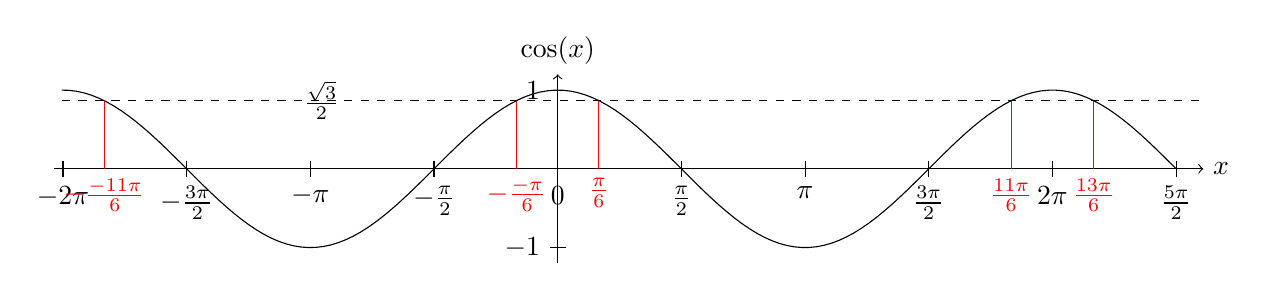
\begin{tikzpicture}[domain=-6.3:7.85]
  \draw[->] (-6.4,0) -- (8.2,0) node[right] {$x$};
  \draw[->] (0,-1.2) -- (0,1.2) node[above] {$\cos(x)$};
  \draw plot [samples=150] (\x,{cos(\x r)});

  \foreach \x/\xtext in {-2*pi/-2\pi, -1.5*pi/-\frac{3\pi}{2},-pi/-\pi, -0.5*pi/-\frac{\pi}{2}, 0,0.5*pi/\frac{\pi}{2}, pi/\pi, 1.5*pi/\frac{3\pi}{2}, 2*pi/2\pi, 2.5*pi/\frac{5\pi}{2} }
    \draw (\x,0.1) -- (\x,-0.1) node[anchor=north] {$\xtext$};

  \foreach \y/\ytext in {-1,1}
    \draw (0.1,\y) -- (-0.1,\y) node[anchor=east] {$\ytext$};

  \draw [dashed] (-6.3, 0.866) -- (8.2,0.866);
  \node (c) at (-3,0.866) {$\frac{\sqrt{3}}{2}$};

  \draw [red] (6.8068, 0.866) -- (6.8068,0) node [below] {$\frac{13\pi}{6}$} ;
  \draw [red] (5.7596, 0.866) -- (5.7596,0) node [below] {$\frac{11\pi}{6}$} ;
  \draw [red] (0.5235, 0.866) -- (0.5235,0) node [below] {$\frac{\pi}{6}$} ;
  \draw [red] (-0.5235, 0.866) -- (-0.5235,0) node [below] {$-\frac{-\pi}{6}$} ;
  \draw [red] (-5.7596, 0.866) -- (-5.7596,0) node [below] {$-\frac{-11\pi}{6}$} ;

\end{tikzpicture}
\end{document}
